  \documentclass[14pt]{beamer}
\usepackage[utf8]{inputenc}
\usepackage{amsmath}
\usepackage{amsfonts}
\usepackage{amssymb}
 \usepackage[compat=1.0.0]{tikz-feynman}
\institute{Instituto de Ciencias Nucleares, UNAM}
\author{José Antonio García Hernández}
\title{El perfil de cuerdas cósmicas no estándares}
%\setbeamercovered{transparent} 
\setbeamertemplate{navigation symbols}{} 
\setbeamertemplate{footline}[frame number]
\usepackage{tikz}
%\logo{} 
%\institute{} 
\date{{\large Seminario de GTD} \\ 27 de abril, 2023} 
%\subject{} 
\begin{document}

\begin{frame}
\titlepage
\end{frame}

\section{Defectos topológicos}
\begin{frame}{Defectos topológicos}
Defecto topológico: singularidad que no puede ser removida sin afectar el campo a largas distancias. \\~\

Muy estable.\\~\

Los tipos de defectos topológicos que puede presentar un sistema se analizan estudiando la topología de la variedad de vacío $\mathcal{M}$.\\~\


\end{frame}

\begin{frame}
Estudiamos sus grupos de homotopía $\pi_n(\mathcal{M})$.\\~\

$\pi_n(\mathcal{M})$: cuenta de cuantas maneras un \textit{loop} de $n$ dimensiones no puede contraerse a un punto. \\~\

Si $\pi_n(\mathcal{M}) \neq I \Rightarrow $ defectos topológicos. \\~\

Si $\pi_n(\mathcal{M}) = \mathbb{Z} \Rightarrow $ carga topológica (\textit{winding number}).
\end{frame}


\begin{frame}{Ejemplos}
Ejemplos:\\
\begin{itemize}
	\item $\pi_0(\mathcal{M}) \neq I \Rightarrow$ Pared de dominio (domain wall). 
	\item $\pi_1(\mathcal{M}) \neq I\Rightarrow$ Vórtice (2d), cuerdas cósmicas (3d)
	\item $\pi_2(\mathcal{M}) \neq I\Rightarrow$ Monopolo  
\end{itemize}
\end{frame}


\begin{frame}
	Existen varios ejemplos de defectos topológicos en la física de materia condensada.\\~\
	
	Pero en la física del universo temprano aun son objetos hipotéticos.
\end{frame}

\begin{frame}
\begin{figure}
\centering
	\includegraphics[scale=0.4]{/home/jose/Documents/Maestria/thesis/chapters/figures/vortexnematics.png}
	\caption{Vórtices en un nemático.}
	\label{fig:vortexnematic}
\end{figure}
\end{frame}

\begin{frame}
\begin{figure}
	\centering
	\includegraphics[scale=0.3]{/home/jose/Documents/Maestria/thesis/chapters/figures/hevortices.png}
	\caption{Vortices cuánticos en gotas de $^4$He superfluido.}
	\label{fig:heliumvortices}
\end{figure} 
\end{frame}


\begin{frame}{Mecanismo de Kibble}
Se asume que hubo transiciones de fase en las ultimas etapas de inflación, en las cuales pudieron haberse creado defectos topológicos. \\~\


\end{frame}



\section{Cuerdas Cósmicas}
\begin{frame}{Cuerdas Cósmicas}
\begin{figure}
	\centering
	\includegraphics[scale=0.4]{/home/jose/Documents/Maestria/thesis/chapters/figures/string.pdf}
	\caption{Vórtices de dos dimensiones uno encima de otro, formando una cuerda en tres dimensiones.}
	\label{fig:string}
\end{figure}
\end{frame}

%\subsection{Cuerdas globales}
%\begin{frame}{Cuerdas cósmicas globales}
%	Lagrangiano euclidiano con $\phi(x) \in \mathbb{C}$
%	\[\mathcal{L} = \frac{1}{2}\partial^{\mu}\phi^*\partial_{\mu} \phi \underbrace{-\frac{m^2}{2}|\phi|^2 - \frac{\lambda}{4}|\phi|^4}_{-V(|\phi|)}\] 
%	con
%	\begin{itemize}
%		\item $m^2 < 0$ 
%		\item $\lambda > 0$
%		\item $v = \sqrt{-\frac{m^2}{\lambda}}$ después del rompimiento espontáneo de la simetría U(1).
%	\end{itemize}
%	
%\end{frame}
%\begin{frame}{Ecuaciones de movimiento}
%	\[ \partial^{\mu}\partial_{\mu}\phi + m^2 \phi + \lambda |\phi|^2\phi = 0.\]
%	Condiciones de frontera
%	\[\lim_{\rho \to 0} \phi = 0, \ \ \ \lim_{\rho \to \infty} |\phi| = v .\]
%	Implica que %bajo las transformaciones $\varphi \to \varphi + \alpha$ el campo se comporta como 
%	$$\phi(\rho,\varphi + \alpha,z) = e^{in\alpha}\phi(\rho,\varphi,z)$$
%	$$\rho \in [0,\infty), \ \ \ \varphi \in (0,2\pi], \ \ \ z \in (-\infty,\infty)$$ 
%	donde $n\in\mathbb{Z}$ es la carga topológica.  
%\end{frame}
%
%\begin{frame}{Ansatz}
%	Ansatz estático en coordenadas cilíndricas
%	\[ \phi(\rho,\varphi) = f(\rho)e^{in\varphi}. \]
%	Ecuación de movimiento para $f$
%	\[\partial_{\rho}^2 f + \frac{1}{\rho}\partial_{\rho}f - \frac{n^2}{\rho^2} f - m^2 f - \lambda f^3 = 0. \]
%	Condiciones de frontera
%	\[f(0) = 0, \ \ \ \lim_{\rho \to \infty} f(\rho) = v .\]
%	Sin solución analítica pero solubles numéricamente.
%\end{frame}
%
%\begin{frame}{Perfil de cuerda cósmica global y densidad de energía}
%	\centering
%	\includegraphics[scale=.85]{global_str.pdf}
%\end{frame}

%\begin{frame}{Cuerdas cósmicas locales}
%Lagrangiano con simetría U(1) local
%\[\mathcal{L} = \frac{1}{2}D^{\mu}\phi^*D_{\mu} \phi - \frac{1}{4}F^{\mu\nu}F_{\mu\nu} - V(|\phi|) \] 
%donde
%\begin{itemize}
%	\item $D_{\mu} \equiv \partial_{\mu} + i h A_{\mu} $
%	\item $F_{\mu\nu} = \partial_{\mu}A_{\nu} - \partial_{\nu}A_{\mu}$
%	\item $V(|\phi|) = \frac{m^2}{2}|\phi|^2 + \frac{\lambda}{4}|\phi|^4 $
%\end{itemize}
%\end{frame}
%
%
%\begin{frame}{Ecuaciones de movimiento. Simetría local}
%Ecuaciones de movimiento
%\begin{eqnarray*}
%	D^{\mu}D_{\mu}\phi & = & -m^2 \phi - \lambda |\phi|^2\phi \\
%	D^{\mu} F_{\mu\nu} & = & -\frac{ih}{2}\left[(D_{\nu}\phi)^*\phi - \phi^*D_{\nu}\phi \right]
%\end{eqnarray*}
% 
%Ansatz estático en coordenadas cilíndricas
%\begin{eqnarray*}
%\phi(r,\varphi) & = & f(r)e^{in\varphi} \\
%A(r) & = & \frac{a(r)}{r} \hat{\varphi},
%\end{eqnarray*}
%donde $n\in\mathbb{Z}$.
%\end{frame}
%
%\begin{frame}{Ecuaciones de movimiento}
%	\begin{eqnarray*}
%		\partial_{r}^2 f + \frac{1}{r}\partial_{r}f - \frac{(n+ha)^2}{r^2} f - m^2 f - \lambda f^3 = 0\\
%		\partial_{r}^2 a - \frac{1}{r}\partial_{r}a - hnf^2 - h^2 a f^2 = 0 \\ 
%	\end{eqnarray*}
%	Condiciones de frontera
%	\begin{eqnarray*}
%		f(0) = 0, & \displaystyle\lim_{r \to \infty} f(r) = v \\
%		a(0) = 0, & \displaystyle\lim_{r \to \infty} a(r) = -\frac{n}{h}
%	\end{eqnarray*}
%\end{frame}
%
%\subsection{Cuerdas locales}
%\begin{frame}{Perfil de cuerda cósmica local, campo de norma y densidad de energía}
%	\centering
%	\includegraphics[scale=.85]{local_str.pdf}
%\end{frame}


\section{Cuerdas cósmicas locales U(1)$_{B-L}$}
\begin{frame}{Simetría global exacta U(1)$_{B-L}$}
En el modelo estándar la simetría U(1)$_{B-L}$ es global y exacta. $B$ número bariónico, $L$ número leptónico.\\~\

Extraño: una simetría exacta solo es natural cuando es local, i.e una simetría de norma. \\~\
\end{frame}

\begin{frame}{Simetría de norma}
Promovemos U(1)$_{B-L}$ global a U(1)$_{B-L}$ local. La combinamos con U$(1)_Y$. \\~\

Introducimos un nuevo acoplamiento de norma $h'$. Definimos a la nueva carga como
	$$Y' = 2hY + \frac{h'}{2}(B-L).$$
Tomamos como grupo de norma a U(1)$_{Y'}$.\\~\

El campo de norma $\mathcal{A}_{\mu}$ es introducido para implementar la invarianza de U$(1)_{Y'}$. \\~\

\end{frame}




\begin{frame}{Anomalía de norma}
\begin{figure}
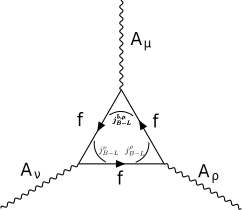
\includegraphics[scale=1]{/home/jose/Documents/Maestria/thesis/chapters/figures/triangularanomaly.pdf}

\caption{En cada vértice  los quarks de una generación contribuyen con $B=4$, y los leptones con $L=3$. $B-L\neq 0$.}
\end{figure}
\centering

\end{frame}

\begin{frame}%{Propiedades de $\mathcal{A}_{\mu}$}

Anomalía de norma. Se cura añadiendo un neutrino derecho $\nu_R$ ($L=1$) a cada generación. \\~\

Podemos dar masa a los neutrinos con un término masa de Dirac
$$ f_{\nu} \left[\bar{\nu}_R \begin{pmatrix}-\Phi_0 & \Phi_+\end{pmatrix}\begin{pmatrix}
	\nu_L \\
	e_L
\end{pmatrix} + \begin{pmatrix}\bar{\nu}_L & \bar{e}_L\end{pmatrix}
\begin{pmatrix}
	-\Phi^*_0 \\
	\Phi^*_+
\end{pmatrix}\nu_R\right], $$
con $f_{\nu}$ un acoplamiento de Yukawa.

\end{frame}


\begin{frame}
Sin promover U$(1)_{B-L}$ a una simetría de norma podemos dar masa a los neutrinos con un término de masa de Majorana
$$	M\bar{\nu}_M \nu_M. $$
Sin embargo, en nuestro escenario, este término está prohibido ya que rompe la simetría U$(1)_{Y'}$.
\end{frame}


\begin{frame}
Para introducir un término de masa tipo Majorana solo para $\nu_R$, independiente de $\nu_L$, introducimos un nuevo campo de Higgs $\chi\in\mathbb{C}$
$$f_{\nu_R} \nu_R^T \chi \nu_R + \text{c.c.},$$
donde $f_{\nu_R}$ es un acoplamiento de Yukawa. \\~\

Para preservar la invarianza de norma, el campo $\chi$ debe tener una carga $B-L=2$.
\end{frame}

\begin{frame}
Generamos la masa de Majorana por el mecanismo de Higgs usando el nuevo campo de Higgs $\chi \in \mathbb{C}$ .\\~\

Llamamos $v'$ al valor esperado del vacío de $\chi$. \\~\

$\chi$ genera una masa de Majorana para el neutrino derecho $M = f_{\nu_R} v'$.  \\~\

\end{frame}

\begin{frame}

$\chi$ se introduce en el Lagrangiano con

$$V' = \frac{m'^{2}}{2}\chi^*\chi+\frac{\lambda'}{4}(\chi^*\chi)^2.$$ 

Es natural incluir un término mixto del tipo 
$$ \frac{\kappa}{2}\Phi^{\dagger}\Phi\chi^*\chi.$$

Asumimos  $v'\gg v$ y $f_{\nu_R}\simeq O(1)$ que da una masa grande al neutrino derecho.
\end{frame}

\subsection{Lagrangiano}
\begin{frame}{Lagrangiano}
\begin{eqnarray*} 
\mathcal{L} & = & \frac{1}{2}(D^{\mu}\Phi)^{\dagger}D_{\mu}\Phi - \frac{m^2}{2}\Phi^{\dagger}\Phi - \frac{\lambda}{4}(\Phi^{\dagger}\Phi)^2 -\frac{\lambda}{4}v^4   \nonumber\\
 & & +\frac{1}{2}(D^{\mu} \chi)^*D_{\mu} \chi - \frac{m'^2}{2}\chi^*\chi - \frac{\lambda'}{4}(\chi^* \chi)^2 -\frac{\lambda'}{4}v'^4\nonumber \\ 
 & & -\frac{\kappa}{2}\Phi^\dagger\Phi\chi^*\chi  -\frac{\kappa}{2}v^2v'^2 -\frac{1}{4}\mathcal{F}^{\mu\nu}\mathcal{F}_{\mu\nu}, %+ \frac{1}{4}B_{\mu\nu}B_{\mu\nu}
\end{eqnarray*}

\begin{itemize}
	\item $\Phi = (\phi_+,\phi_0)^{\text{T}} \in \mathbb{C}^2$
	\item $D_{\mu} \Phi = (\partial_{\mu} + ih\mathcal{A}_{\mu})\Phi$
	\item $D_{\mu} \chi = (\partial_{\mu} + ih'\mathcal{A}_{\mu})\chi$
\end{itemize}
\end{frame}

\begin{frame}


Los campos transforman de la siguiente manera
\begin{eqnarray*}
	\Phi(x) \to e^{ih\alpha(x)}\Phi(x), \nonumber \\
	\chi(x) \to e^{ih'\alpha(x)}\chi(x), \nonumber\\
	\mathcal{A}_{\mu} \to \mathcal{A}_{\mu} + \partial_{\mu} \alpha(x),
\end{eqnarray*}
donde $\alpha(x)$ es cualquier función diferenciable de $x$.
\end{frame}

\begin{frame}
Para que el potencial esté acotado por abajo necesitamos que
\begin{equation*}
	\lambda>0, \ \ \ \lambda'>0, \ \ \ \kappa^2 < \lambda \lambda',
\end{equation*}
y para que ocurra un rompimiento espontáneo de simetría
\begin{equation*}
 m^2 = -\kappa v'^2 - \lambda v^2<0,\ \ \ m'^2 = -\kappa v^2 - \lambda' v'^2<0.
\end{equation*}

\end{frame}

\begin{frame}{Ecuaciones de movimiento}
\begin{eqnarray*}
	D^{\mu}D_{\mu} \Phi & = & -m^2 \Phi - \lambda (\Phi^{\dagger}\Phi)\Phi - \kappa \Phi \chi^* \chi \\
	D^{\mu}D_{\mu} \chi & = & -m'^2 \chi - \lambda' (\chi^{*}\chi)\chi - \kappa \chi \Phi^{\dagger} \Phi \\
	\partial^{\lambda}\mathcal{F}_{\lambda\nu}  & = & -\frac{ih}{2}\left[ (D_{\nu}\Phi)^{\dagger}\Phi-\Phi^{\dagger}(D_{\nu}\Phi)\right] \\
	& & - \frac{ih'}{2}\left[ (D_{\nu}\chi)^{*}\chi-\chi^{*}(D_{\nu}\chi)\right]
\end{eqnarray*}
\end{frame}

\begin{frame}{Ansatz}

$\mathcal{M} = \text{U}(1) \Rightarrow \pi_1(\text{U}(1)) = \mathbb{Z} \Rightarrow$ cuerdas cósmicas. \\~\

Solo consideramos la componente $\phi_0$ del campo de Higgs $\Phi$. \\~\

Ansatz cilíndrico y estático

\begin{eqnarray*}
	\phi_0(r,\varphi) & = & \phi(r) e^{in\varphi} \\
	\chi(r,\varphi) & = & \xi(r) e^{in'\varphi} \\
	\mathbf{\mathcal{A}}(r) & = & \frac{a(r)}{r} \hat{\varphi}.
\end{eqnarray*}

\end{frame}
\subsection{Ecuaciones de movimiento}
\begin{frame}{Ecuaciones de movimiento}
\begin{eqnarray*}
\partial_r^2 \phi + \frac{1}{r} \partial_r \phi- \frac{\left(n+ha\right)^2}{r^2}\phi- m^2 \phi- \lambda \phi^3-\kappa \phi \xi^2 = 0 \\
\partial_r^2 \xi + \frac{1}{r} \partial_r \xi - \frac{\left(n'+h'a\right)^2}{r^2}\xi -m'^2\xi - \lambda' \xi^3 -\kappa \xi \phi^2 = 0\\
\partial_r^2a -\frac{1}{r}\partial_r a-h(n+ha)\phi^2-h'(n' + h'a )\xi^2 = 0.
\end{eqnarray*}
Condiciones de frontera
\begin{eqnarray*}
	\phi(0)=0, & \displaystyle\lim_{r\to\infty}\phi(r) = v \\
	 \xi(0)=0, &  \displaystyle\lim_{r\to\infty}\xi(r) = v' \\
	 a(0)=0, & \displaystyle \lim_{r\to\infty}a(r) = -\frac{n}{h}=-\frac{n'}{h'} .
\end{eqnarray*}
Condiciones de frontera
\end{frame}

\begin{frame}

Problema  con condiciones a la frontera, soluciones numéricas con el método de Newton amortiguado.\\~\

Las soluciones están definidas de manera única al definir $v$, $v'$, $\lambda$, $\lambda'$, $h$, $h'$, $n$ y $n'$.\\~\

Escogimos $v'\gg v$. \\~\

$v=246$ GeV se usa para convertir a todas las variables adimensionales a unidades físicas.
\end{frame}


 \begin{frame}
Mostramos el radio $r$ del perfil en unidades de 
 
 \begin{equation*}
	 v_{\text{dim'less}} \ 0.0008 \ \text{fm}.
\end{equation*}


 \end{frame}

\subsection{Resultados}


\begin{frame}
\begin{figure}
	\centering
	\includegraphics[scale=0.6]{/home/jose/Documents/Maestria/thesis/chapters/figures/F0.pdf}
	\caption{$v=0.5$, $v'=1$, $n=n'=h=h'=\lambda=\lambda'=1$.}
\end{figure}
\end{frame}

\begin{frame}
\begin{figure}
	\centering
	\includegraphics[scale=0.6]{/home/jose/Documents/Maestria/thesis/chapters/figures/Figure_1.pdf}
	\caption{$v = 0.5$, $v'=1$, $n=1$, $n'=2$, $h=1$, $h'=2$, $\lambda=\lambda'=1$.}
\end{figure}
\end{frame}

\begin{frame}
\begin{figure}
	\centering
	\includegraphics[scale=0.6]{/home/jose/Documents/Maestria/thesis/chapters/figures/n-5h5np-1hp1l1lp1v05vp2.pdf}
	\caption{$v = 0.5$, $v'=2$, $n=-5$, $n'=-1$, $h=5$, $h'=1$, $\lambda=\lambda'=1$. This is an example from the SO(10) model.}
	\label{fig:n-5h5np-1hp1l1lp1v05vp2}
\end{figure}
\end{frame}

\begin{frame}
\begin{figure}
	\centering
	\includegraphics[scale=0.6]{/home/jose/Documents/Maestria/thesis/chapters/n1h1np1hp1l1lp1v001vp1edited.pdf}
		\caption{$n = h = n' = h'  = \lambda=\lambda' = 1,\ v =0.01,\ v' = 1 $.}
		\label{fig:sol1}
\end{figure}
\end{frame}

\begin{frame}
\begin{figure}
	\centering
	\includegraphics[scale=0.59]{/home/jose/Documents/Maestria/thesis/chapters/n-2h05np10hp-25l1lp1v001vp1combined.pdf}
		\caption{$n = -2,\ h =0.5,\ n' = 10,\ h' = -2.5,\  \lambda=1,\ \lambda' = 1,\ v =0.01,\ v' = 1 $.}
		\label{fig:coaxial}
\end{figure}
\end{frame}


\begin{frame}
\begin{figure}
	\centering
	\includegraphics[scale=.5]{/home/jose/Documents/Maestria/thesis/chapters/figures/n-2h05np10hp-25l1lp1v001vp1eden.pdf}
	\caption{Densidad de energía, $v = 0.01$, $v'=1$, $n=-2$, $n'=10$, $h=0.5$, $h'=-2.5$, $\lambda=\lambda'=1$. En unidades de $4.79\times 10^{19}\ \text{GeV}/\text{fm}^3$.}
	\label{fig:edencoaxial}
\end{figure}
\end{frame}

\begin{frame}
Al integrar la densidad de energía encontramos que la tensión de las cuerdas estan en el orden de
\begin{equation*}
	\mu \sim 10^{10}\ \text{GeV}^2.
\end{equation*}

%\begin{equation*}
%	G\mu \sim  10^{-28}.
%\end{equation*}

\end{frame}



\begin{frame}{Busqueda de cuerdas cósmicas}
Introducimos la variable adimensional
\begin{equation*}
	G\mu ,
\end{equation*}
donde $\mu$ es la tensión de la cuerda y $G = \frac{1}{(1.2\times 10^{19}\ \text{GeV})^2}$ es la constante de Newton.\\~\

Mide, por ejemplo, el acoplamiento gravitacional de la cuerda.
\end{frame}


\begin{frame}{Mediciones del power spectrum del CMB}

Justo después del \textit{Big Bang} el universo estaba permeado de un plasma de bariones, leptones y fotones.\\~\

Cuando el universo tenia $\sim 300,000$ años, los primeros atomos fueron formados. \\~\

Dado que los átomos son neutros, los fotones se desacoplaron de la materia. Un proceso llamado \textit{recombinación}.\\~\

Esta radiación es llamada CMB.

\end{frame}

\begin{frame}
	Si las cuerdas cósmicas existen, tendrían una huella distintiva en el \textit{power spectrum} del CMB.\\~\
	
La radiación que pasa cercana a una cuerda cósmica causaría que las discontinuidades en la desviación de la temperatura del CMB sea del orden
\begin{equation*}
	\frac{\Delta T}{T} = 8\pi G \mu \beta,
\end{equation*}	
	donde $\beta$ es la velocidad transeversal de la cuerda, $T$ es la temperatura promedio y $\Delta T$ es la fluctuacion de la temperatura.
\end{frame}

\begin{frame}
\begin{figure}
	\centering
	\includegraphics[scale=0.45]{/home/jose/Documents/Maestria/thesis/chapters/figures/Planck_Power_Spectrum.jpg}
\end{figure}
\end{frame}


\begin{frame}
De acuerdo a las mediciones del CMB obtenidas por PLANCK, la constricción para la tensión de la cuerda es
\begin{equation*}
G\mu \lesssim 1.49\times 10^{-7}.
\end{equation*}
\end{frame}


\begin{frame}{Lentes gravitacionales}
Tensor energía momento de una cuerda cósmica estática
\begin{equation*}
	T^{\mu\nu} = \mu\delta(x)\delta(y)\,\text{diag}(1,0,0,-1).
	\label{eq:energytensor}
\end{equation*}
Lejos de la cuerda el elemento de línea es
\begin{equation*}
	ds^2 = dt^2-dr'^2-r'^2d\varphi'^2-dz^2,
	\label{eq:metric}
\end{equation*}
donde 
\begin{equation*}
(1-8G\mu\log(r/r_0))r^2 = (1-8G\mu)r^2,  \ \varphi' = (1-4G\mu)\varphi.
\end{equation*}
Aquí $r\in [0,\infty] $ y $\varphi\in[0,2\pi)$ y $r_0$ es una constante.
\end{frame}


\begin{frame}
 Esto implica una deficit angular 
\begin{equation*}
\Delta \varphi = \varphi_{\text{max}} - \varphi'_{\text{max}} = 2\pi -2\pi(1-4G\mu) = 8\pi G\mu.
\end{equation*}
Un objeto detrás de una cuerda cósmica produce dos objetos similares separados por el ángulo
\begin{equation*}
	\alpha = \frac{l_1}{l_2}\Delta\varphi\sin\theta,
\end{equation*}
asumiendo $G\mu\ll 1$, donde $l_1$ es la distancia entre la cuerda y el observador, $l_2$ es la distancia entre la cuerda y el objeto y $\theta$ es el ángulo que hace la cuerda con un plano perpendicular entre el observador y el objeto. 
\end{frame}

\begin{frame}
\begin{figure}
	\centering
	\includegraphics[scale=0.3]{/home/jose/Documents/Maestria/thesis/chapters/figures/stringlensing.jpeg}
\end{figure} 
\end{frame}


\begin{frame}{Ondas gravitacionales}
Una de  las formas más realistas de detectar cuerdas cósmicas es por su emisión de ondas gravitacionales.\\~\

De acuerdo a la Relatividad General, un \textit{loop} oscilante de cuerda cósmica emite radiación gravitacional con una potencia
\begin{equation*}
	P = \gamma G \mu^2.
\end{equation*}

\end{frame}

\begin{frame}

	Estos \textit{loops} tienen una emisión característica de radiación gravitacional producidas por \textit{kinks} y \textit{cúspides}.\\~\

	Los kinks son discontinuidades en $\dot x^{\mu}$. \\~\

	Las cúspides son regiones puntiagudas del loop.\\~\
	
	Las cúspides producen señales de ondas gravitacionales en la dirección del pico.
	
\end{frame}

\begin{frame}
	\begin{figure}
	\centering
	\includegraphics[scale=1.5]{/home/jose/Documents/Maestria/thesis/chapters/figures/cusp.pdf}
	\caption{A loop with a cusp. Near the cusp the speeds of the right and left modes are the speed of light.}
		\label{fig:cusp}
\end{figure}
\end{frame}

\begin{frame}
	La colaboración LIGO/VIRGO han puesto constricciones a la tension de las cuerdas.\\~\
	
	 Refiriendose a radiación por loops, la constricción de la tensión es
	\begin{equation*}
		G\mu \lesssim 4\times 10^{-15}.
	\end{equation*}		
	
\end{frame}

\section{Conclusiones}
\begin{frame}{Conclusiones}
En esta extensión del MS hemos introducido
\begin{itemize}
	\item Un nuevo acoplamiento de norma $h'$ 
	\item Un neutrino derecho $\nu_R$
	\item Un nuevo campo de Higgs $\chi\in\mathbb{C}$ \\~\

\end{itemize}

%Una partícula cerca de la cuerda podría modificar temporalmente su masa.\\~\

A larga distancia no afecta a la física conocida.\\~\

No observado pero en principio detectable. \\~\

La tensión de las cuerdas es del orden de $10^{10}$ GeV.\\~\

\end{frame}

\begin{frame}

Obtuvimos soluciones tipo \textit{overshoot} y \textit{coaxiales}.\\~\

Es un escenario posible sin contradicciones a la física del modelo estándar.\\~\

Detección difícil, pero no estan descartas con las observaciones actuales.\\~\

Un argumento válido en su favor es la explicación del porqué la invarianza $B-L$ es una simetría exacta.

\end{frame}

%\begin{frame}{Lagrangiano}
%\begin{eqnarray*}
%	\mathcal{L} = (\bar{\nu}_L,\bar{e}_L \gamma_{\mu})D_{\mu}\begin{pmatrix}
%	\nu_L \\
%	e_L
%	\end{pmatrix} + (\bar{u}_L^c,\bar{d}_L^c \gamma_{\mu})D_{\mu}\begin{pmatrix}
%	u_L^c \\
%	d_L^c
%	\end{pmatrix} \\
%	+ \sum_{f = \nu,e,u^c,d^c}\bar{f}_R\gamma_{\mu} d_{\mu} f_R \\
%	f_e (\bar{\nu}_L,\bar{e}_L)\Phi e_R + f_{\nu} (\bar{\nu}_L,\bar{e}_L)\tilde\Phi \nu_R 
%\end{eqnarray*}

%\end{frame}

\end{document}